\documentclass[12pt,a4paper]{article}

% Compilar con pdfLaTeX
\usepackage[spanish,es-nodecimaldot]{babel}
\usepackage[utf8]{inputenc}
\usepackage[T1]{fontenc}
\usepackage{newtxtext,newtxmath}
\usepackage{geometry}
\geometry{margin=2.4cm}
\usepackage{amsmath,amssymb}
\usepackage{booktabs}
\usepackage{float}
\usepackage{enumitem}
\usepackage{microtype}
\usepackage{graphicx}
\usepackage{hyperref}
\hypersetup{colorlinks=true,linkcolor=black,urlcolor=blue}

\title{\textbf{Regresión lineal para la predicción del ingreso mensual}\\
\large Comparación de particiones de entrenamiento y prueba}
\date{\today}

\begin{document}
\maketitle

\begin{abstract}
Este informe estudia la capacidad de una regresión lineal para predecir el ingreso mensual a partir de edad, años de escolaridad, nivel educativo y sexo. Se comparan tres particiones aleatorias de los datos: 80/20, 90/10 y 70/30. La evaluación se realiza sobre observaciones reservadas para prueba y se utilizan el coeficiente de determinación ($R^2$), el error absoluto medio (MAE) y la raíz del error cuadrático medio (RMSE). Los resultados favorecen la partición 80/20 en $R^2$, aunque las diferencias entre proporciones no son concluyentes por sí solas, dado que se utiliza una sola división aleatoria por configuración.
\end{abstract}

\section{Datos y preparación}
Se utilizó la hoja \texttt{Sheet1} del archivo \texttt{data.xlsx}, que contiene $10\,280$ registros y las variables \texttt{edad}, \texttt{nivel\_edu}, \texttt{ingreso\_mensual}, \texttt{sex} y \texttt{anios\_esc}, además de un identificador. La columna \texttt{id} se excluyó de los predictores, porque funciona como identificador y no constituye una característica explicativa del ingreso.

El ingreso mensual se definió como variable objetivo. Los predictores fueron edad, años de escolaridad, nivel educativo y sexo. Las variables numéricas se imputan con la mediana y las categóricas con la categoría más frecuente. Las categorías se codifican mediante variables indicadoras (*one-hot encoding*), omitiendo una categoría de referencia. El preprocesamiento se ajusta dentro de un \textit{pipeline} únicamente con los datos de entrenamiento, para evitar fuga de información desde el conjunto de prueba.

\section{Diseño experimental: proporciones 80/20, 90/10 y 70/30}
Se evaluaron tres divisiones de los datos, manteniendo fija la semilla aleatoria en $42$ para que el experimento sea reproducible. En cada caso, el modelo se entrena con la primera proporción y se evalúa con la fracción restante.

\begin{table}[H]
\centering
\caption{Tamaño de los conjuntos para cada partición}
\begin{tabular}{lrr}
\toprule
\textbf{Partición} & \textbf{Entrenamiento} & \textbf{Prueba}\\
\midrule
80/20 & 8\,224 & 2\,056\\
90/10 & 9\,252 & 1\,028\\
70/30 & 7\,196 & 3\,084\\
\bottomrule
\end{tabular}
\end{table}

No existe una proporción que sea óptima para todos los problemas. La división 80/20 es una convención práctica porque conserva una cantidad amplia de observaciones para estimar el modelo y reserva una muestra de prueba suficientemente grande. La comparación empírica permite valorar si las conclusiones cambian bajo otras proporciones.

\section{Formulación matemática}
Sea $Y_i$ el ingreso mensual de la observación $i$. El modelo múltiple se representa como
\begin{equation}
Y_i=\beta_0+\beta_1 E_i+\beta_2 S_i+
\sum_{j=1}^{J-1}\gamma_jD_{ij}+\delta M_i+\varepsilon_i,
\end{equation}
donde $E_i$ es la edad, $S_i$ son los años de escolaridad, $D_{ij}$ son variables indicadoras de nivel educativo y $M_i$ representa la categoría codificada de sexo. Se omite una categoría de cada variable cualitativa como referencia.

Los coeficientes se estiman mediante mínimos cuadrados ordinarios:
\begin{equation}
\widehat{\boldsymbol{\beta}}=
\arg\min_{\boldsymbol{\beta}}
\sum_{i\in\mathcal{T}}(Y_i-\widehat{Y}_i)^2,
\end{equation}
donde $\mathcal{T}$ denota el conjunto de entrenamiento. Los coeficientes describen asociaciones condicionadas por los demás predictores; no prueban causalidad.

\section{Métricas}
El coeficiente de determinación se calcula como
\begin{equation}
R^2=1-\frac{\sum_{i=1}^{n_{\mathrm{prueba}}}(Y_i-\widehat{Y}_i)^2}
{\sum_{i=1}^{n_{\mathrm{prueba}}}(Y_i-\overline{Y}_{\mathrm{prueba}})^2}.
\end{equation}
El error absoluto medio y la raíz del error cuadrático medio son
\begin{align}
\mathrm{MAE}&=\frac{1}{n_{\mathrm{prueba}}}\sum_i|Y_i-\widehat{Y}_i|,\\
\mathrm{RMSE}&=\sqrt{\frac{1}{n_{\mathrm{prueba}}}\sum_i(Y_i-\widehat{Y}_i)^2}.
\end{align}
Un $R^2$ más alto y valores menores de MAE y RMSE suelen indicar mejor desempeño predictivo. El MAE es el error absoluto promedio, mientras que el RMSE penaliza con mayor fuerza los errores grandes.

\section{Resultados: comparación de particiones}
\begin{table}[H]
\centering
\caption{Desempeño del modelo múltiple en los datos de prueba}
\begin{tabular}{lrrrr}
\toprule
\textbf{Partición} & \textbf{$R^2$} & \textbf{MAE} & \textbf{RMSE}\\
\midrule
80/20 & 0,2784 & 3\,205,94 & 4\,808,47\\
90/10 & 0,2588 & 3\,210,01 & 4\,660,10\\
70/30 & 0,2665 & 3\,168,57 & 4\,904,97\\
\bottomrule
\end{tabular}
\end{table}

La partición 80/20 obtiene el mayor $R^2$ ($0{,}2784$), mientras que 70/30 presenta el menor MAE ($3\,168{,}57$) y 90/10 el menor RMSE ($4\,660{,}10$). Por tanto, no existe un ganador en todas las métricas. El modelo explica aproximadamente el $27{,}84\%$ de la variabilidad del ingreso en la muestra de prueba 80/20; esto representa una capacidad explicativa moderada, no una precisión alta.

Las métricas entre particiones son relativamente cercanas, aunque no idénticas. Cada proporción deja un conjunto de prueba diferente y, por tanto, las métricas también dependen de qué observaciones quedan reservadas. La semilla fija asegura que los resultados puedan reproducirse, pero no convierte una única división en una demostración universal de superioridad.


\begin{figure}[H]
\centering
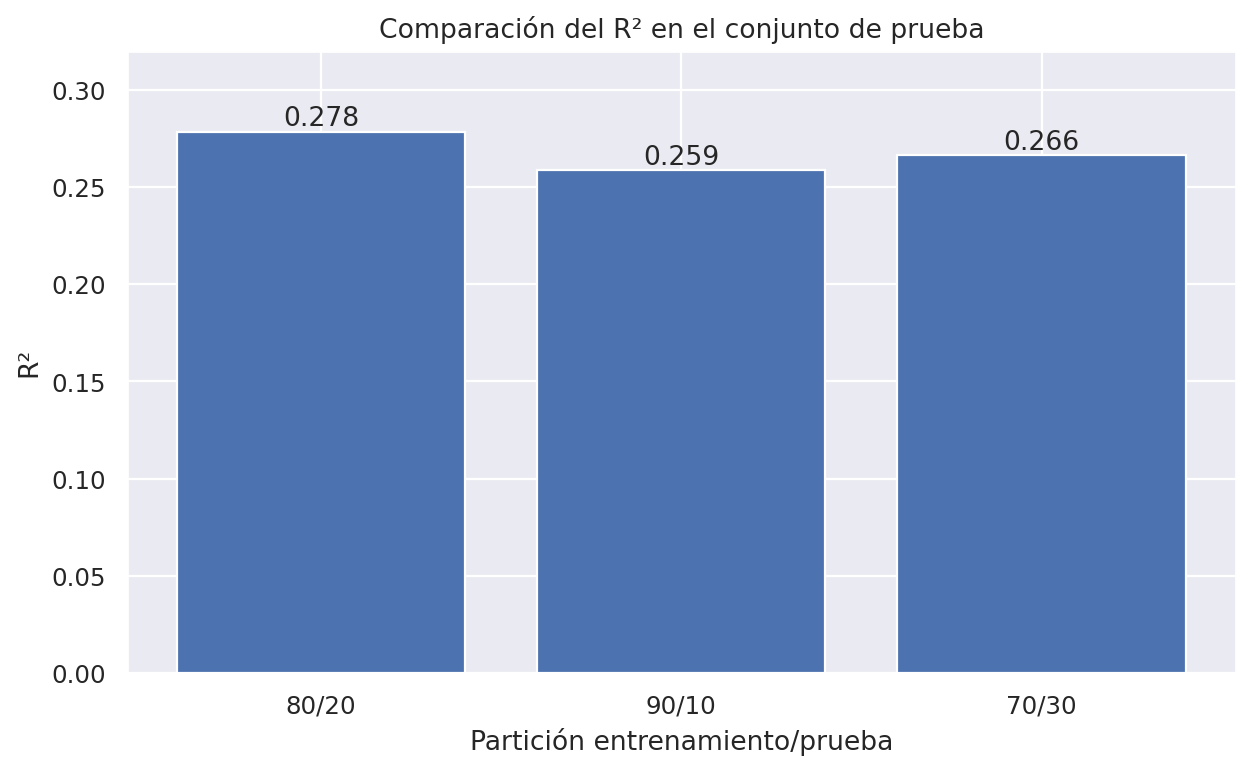
\includegraphics[width=0.78\textwidth]{figures/comparacion_r2.png}
\caption{Comparación del coeficiente de determinación para las tres particiones.}
\label{fig:comparacion-r2}
\end{figure}

\begin{figure}[H]
\centering
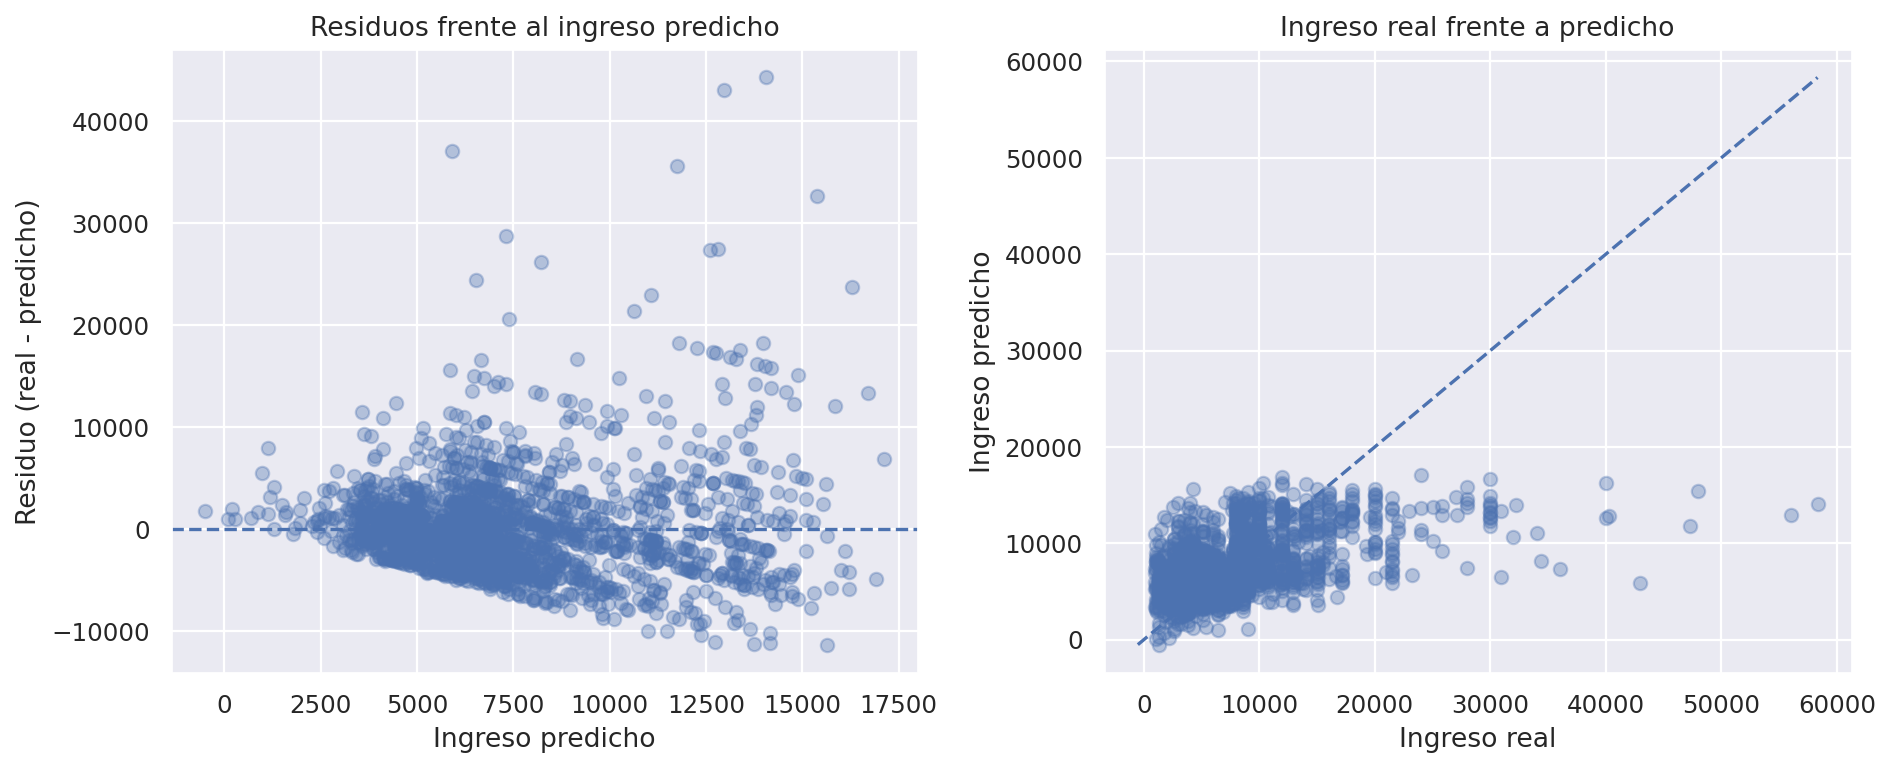
\includegraphics[width=0.95\textwidth]{figures/diagnostico_80_20.png}
\caption{Diagnóstico gráfico del modelo múltiple en la partición 80/20. A la izquierda se muestran los residuos frente a los valores predichos; a la derecha, los ingresos observados frente a los predichos.}
\label{fig:diagnostico}
\end{figure}

\section{Comparación con un modelo que utiliza solo edad}
Como referencia, en la partición 80/20 se comparó el modelo múltiple con una regresión que utiliza únicamente la edad.

\begin{table}[H]
\centering
\caption{Modelo de edad frente al modelo múltiple, con partición 80/20}
\begin{tabular}{lrrr}
\toprule
\textbf{Modelo} & \textbf{$R^2$} & \textbf{MAE} & \textbf{RMSE}\\
\midrule
Solo edad & 0,0015 & 3\,881,45 & 5\,656,31\\
Regresión múltiple & 0,2784 & 3\,205,94 & 4\,808,47\\
\bottomrule
\end{tabular}
\end{table}

La regresión con edad solamente tiene un $R^2$ cercano a cero. Al incluir años de escolaridad, nivel educativo y sexo, el $R^2$ aumenta a $0{,}2784$, y los errores MAE y RMSE disminuyen. Esto sugiere que las variables adicionales mejoran la predicción en esta muestra. No implica que las variables causen cambios en el ingreso, ni que se hayan incluido todos los factores relevantes.

\section{Discusión y limitaciones}
\begin{enumerate}[label=\arabic*)]
\item \textbf{Elección de la proporción.} El 80/20 se puede defender como equilibrio práctico entre entrenamiento y prueba y, en este experimento, obtuvo el mayor $R^2$. No se debe afirmar que es siempre la mejor proporción.
\item \textbf{Una sola división por proporción.} Para evaluar estabilidad, se recomienda repetir el análisis con varias semillas o emplear validación cruzada. Se deben comparar promedios y desviaciones estándar de las métricas.
\item \textbf{Capacidad explicativa.} Incluso el mayor $R^2$ es aproximadamente $0{,}28$, por lo que gran parte de la variabilidad permanece sin explicar.
\item \textbf{Supuestos del modelo.} Se recomienda examinar residuos, heterocedasticidad, valores extremos y posible relación no lineal entre edad e ingreso.
\item \textbf{Representatividad.} El número de registros no garantiza que los datos representen a toda una población. Para generalizar los resultados es necesario conocer el proceso de muestreo y la población de origen.
\end{enumerate}

\section{Conclusiones}
Se compararon las proporciones 80/20, 90/10 y 70/30 manteniendo el modelo y la semilla aleatoria. El 80/20 obtuvo el mayor coeficiente de determinación; sin embargo, 70/30 obtuvo el menor MAE y 90/10 el menor RMSE. La evidencia respalda utilizar 80/20 como configuración principal por equilibrio y por su resultado en $R^2$, pero no demuestra que sea universalmente superior.

La comparación con el modelo que utiliza solo edad indica que incorporar variables educativas y sexo mejora el desempeño predictivo en la división 80/20. Como mejora metodológica, se recomienda realizar validación cruzada o repetir la comparación con distintas semillas para cuantificar la variabilidad de los resultados.

\section*{Reproducibilidad}
El código Python asociado carga \texttt{data.xlsx}, compara las tres proporciones y guarda las métricas y gráficas en la carpeta \texttt{resultados\_regresion}. Los resultados se reproducen usando la semilla aleatoria $42$ y las mismas versiones de las bibliotecas de análisis.

\end{document}
